\begin{figure*}[t]
	\centering
	\begin{tabular}{cccc}
		\hspace{-0.5em}\subfloat[][$\Delta=1\times10^{-2}$]{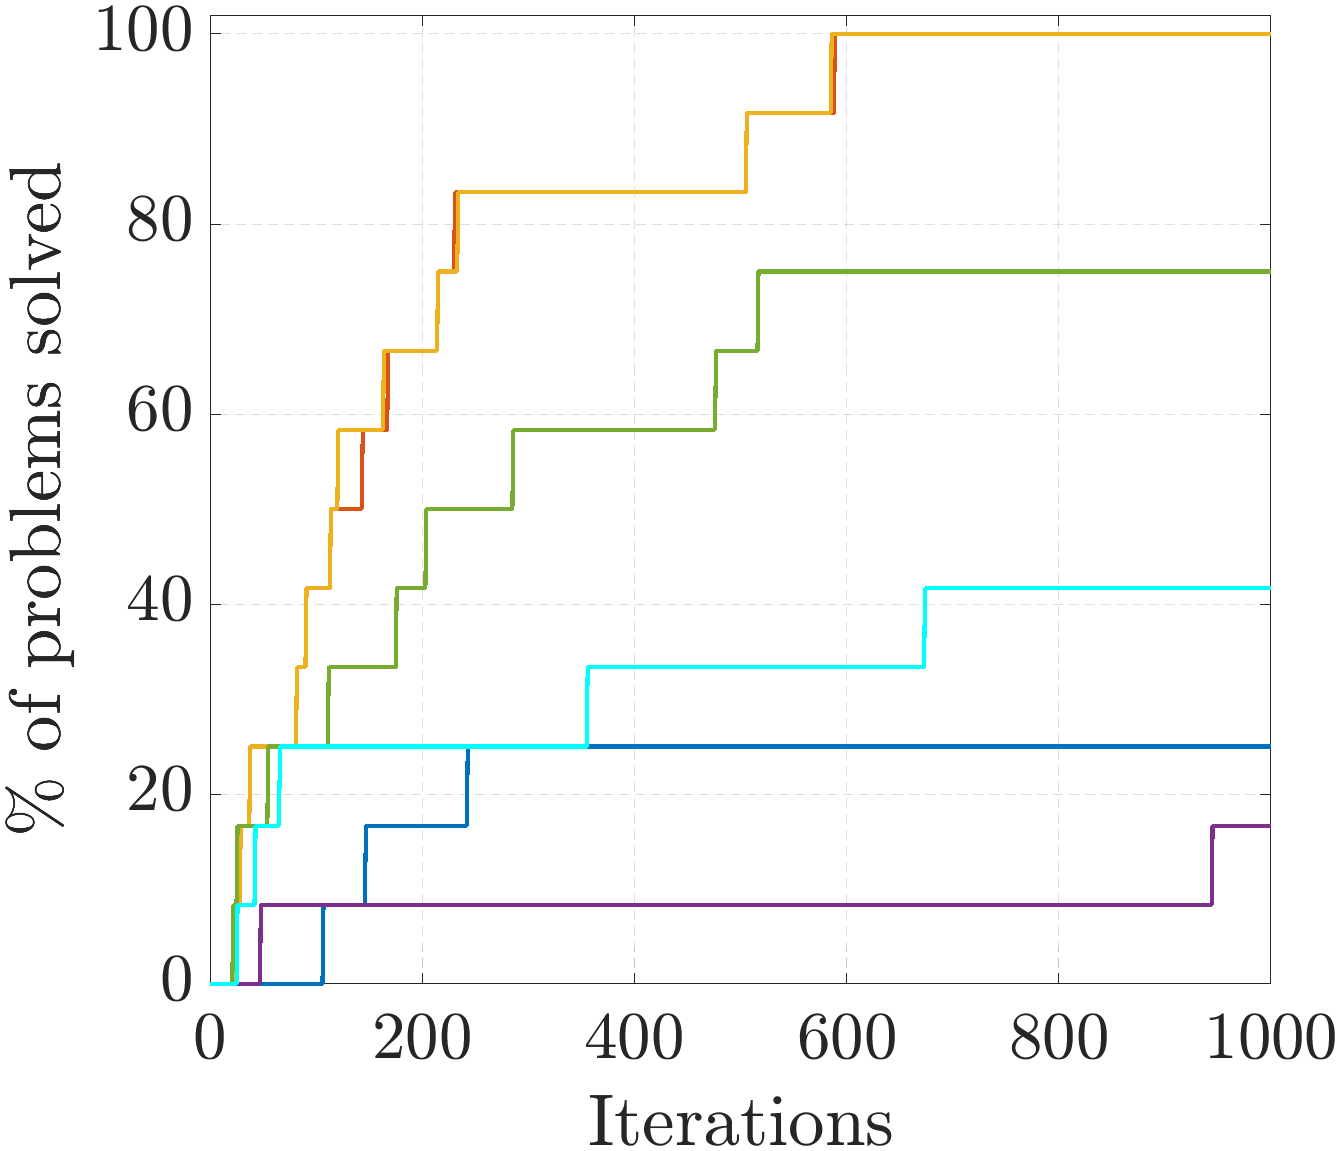
\includegraphics[trim =0mm 0mm 0mm 0mm,width=0.2425\textwidth]{figures/succ/succ_iter_1.png}} &
		\hspace{-0.6em}\subfloat[][$\Delta=5\times10^{-3}$]{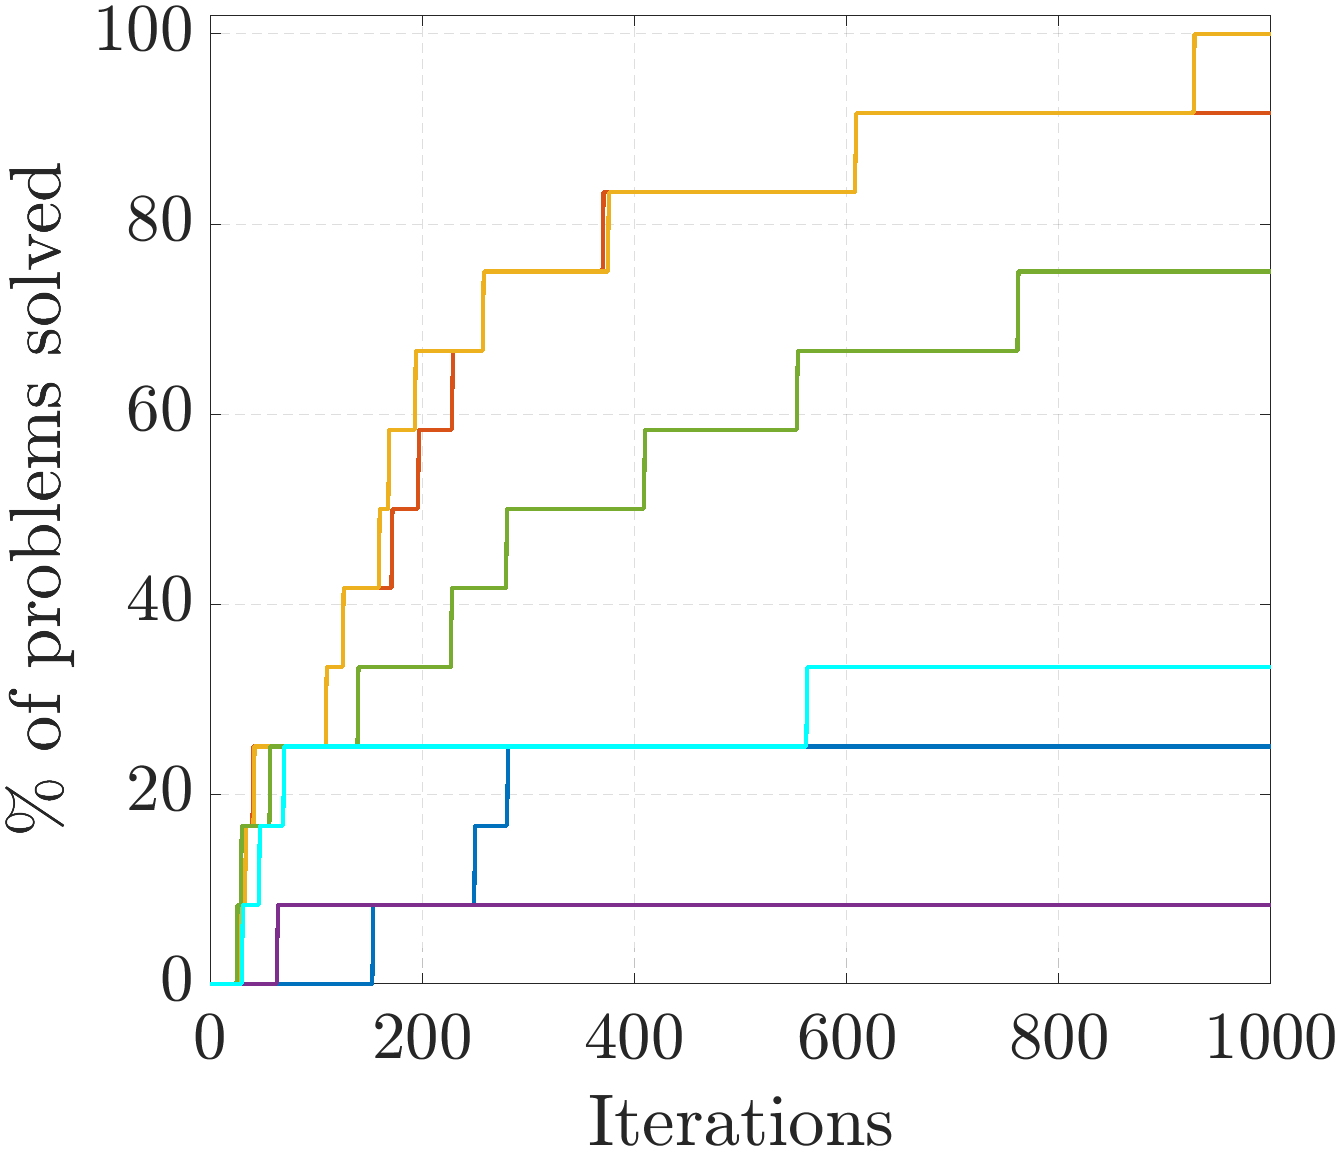
\includegraphics[trim =0mm 0mm 0mm 0mm,width=0.2425\textwidth]{figures/succ/succ_iter_2.png}} &
		\hspace{-0.6em}\subfloat[][$\Delta=1\times10^{-3}$]{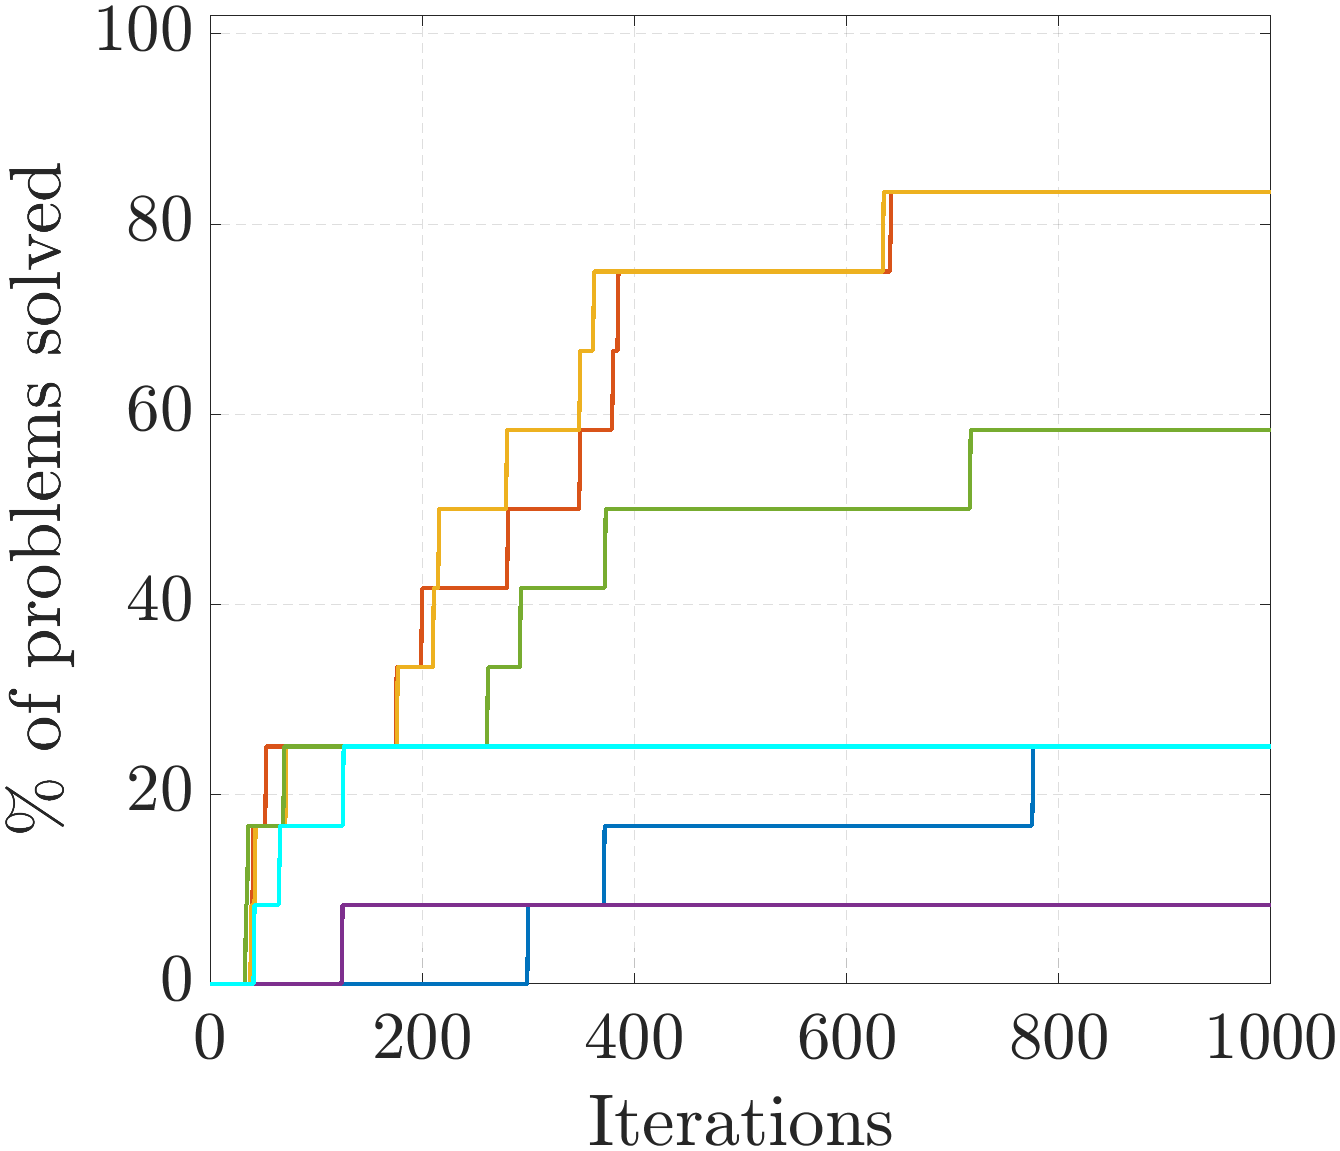
\includegraphics[trim =0mm 0mm 0mm 0mm,width=0.2425\textwidth]{figures/succ/succ_iter_3.png}}&
		\hspace{-0.6em}\subfloat[][$\Delta=1\times10^{-4}$]{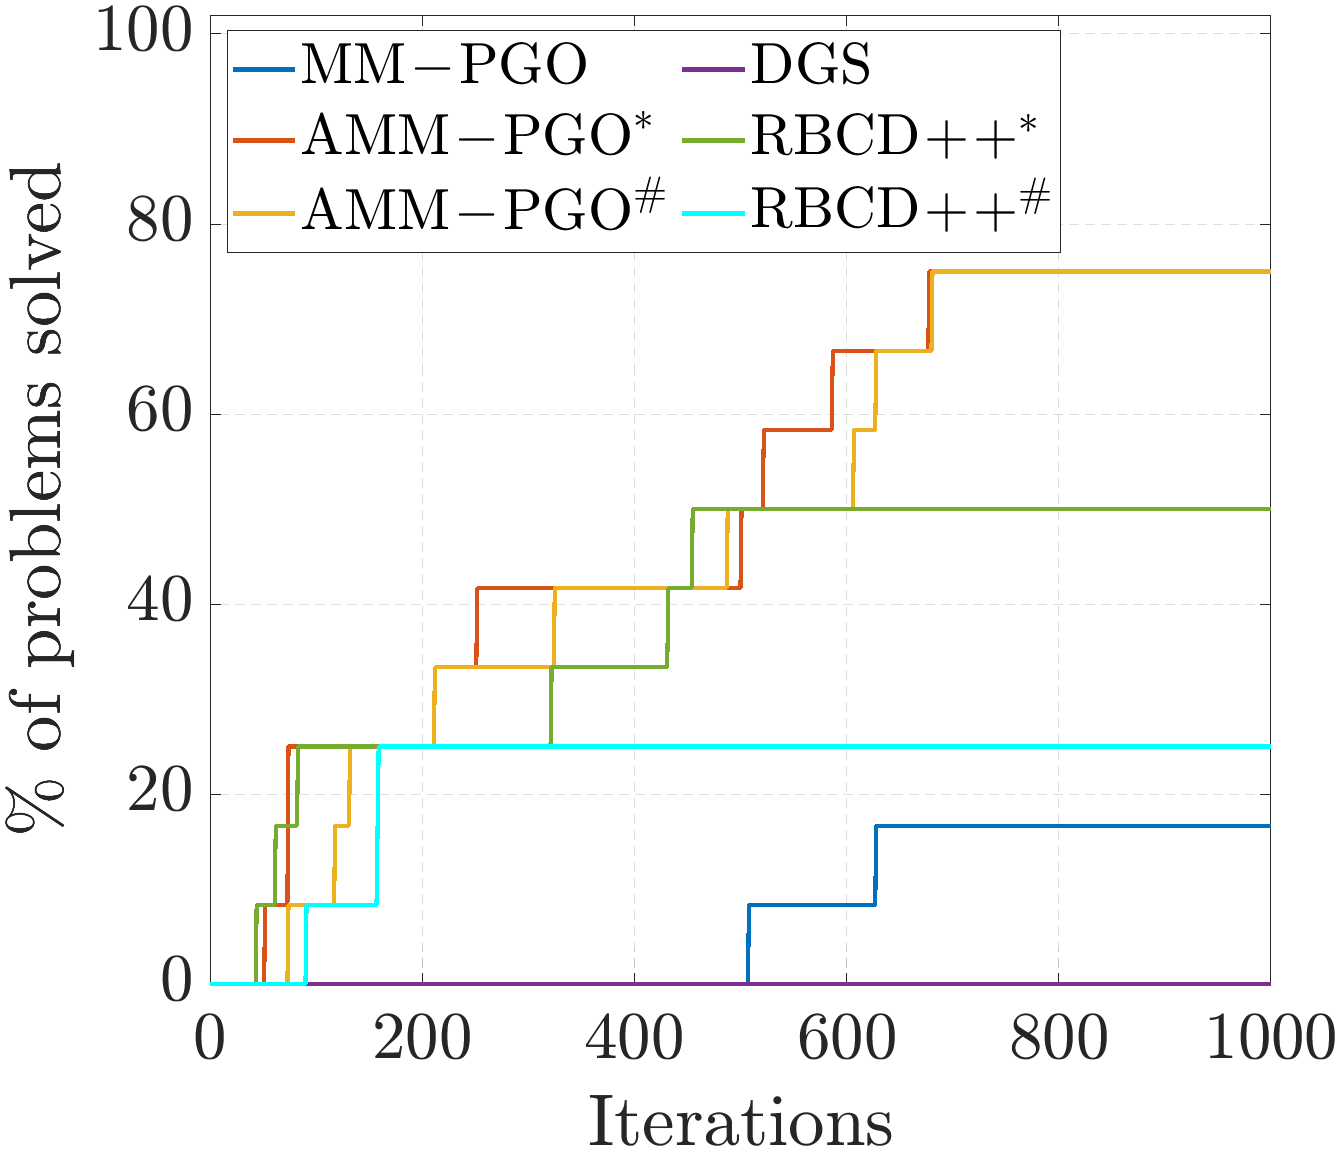
\includegraphics[trim =0mm 0mm 0mm 0mm,width=0.2425\textwidth]{figures/succ/succ_iter_4.png}}
	\end{tabular}
	\caption{Performance profiles for $\mm$, $\ammc$, $\ammd$, $\dgs$ \cite{choudhary2017distributed}, $\rbcdc$ \cite{tian2019distributed} and $\rbcdd$ \cite{tian2019distributed} on 2D and 3D SLAM Benchmark datasets (see \datasetinfo). The performance is based on the number of iterations $\sk$ and the evaluation tolerances are $\Delta=1\times10^{-2}$, $5\times10^{-3}$, $1\times10^{-3}$, $1\times10^{-4}$. The distributed PGO has 10 robots (nodes) and is initialized with distributed Nesterov's accelerated chordal initialization \cite{fan2020mm}. Note that $\ammc$ and $\rbcdc$  require a master node, whereas $\mm$, $\ammd$, $\dgs$  and $\rbcdd$ do not.}\label{fig::succ_iter}
	\vspace{-1em}
\end{figure*}